\clearpage
\chapter{Aprendizado de Máquina}

O aprendizado de máquina tem como objetivo criar técnicas computacionais e sistemas que automaticamente adquirem conhecimento. Existem diversos algoritmos de aprendizado de máquina, utilizados para resolver problemas específicos. É importante, portanto, compreender suas limitações \cite{rezende2003}.

As tarefas de aprendizado de máquina podem ser classificadas em:

\begin{itemize}
    \item \textbf{Aprendizado supervisionado:} é fornecido ao algoritmo um conjunto de entradas e suas respectivas saídas, com o objetivo de aprender uma regra geral que mapeia as entradas às saídas.
    \item \textbf{Aprendizado não-supervisionado:} somente um conjunto de entrada é fornecido, com o objetivo do próprio algoritmo identificar os padrões do conjunto de dados.
    \item \textbf{Aprendizado por estímulo:} o algoritmo interage com o ambiente dinâmico afim de concluir determinados objetivos.
    \item \textbf{Aprendizado semi-supervisionado:} utiliza um conjunto de treinamento que inclui alguns elementos pré-classificados junto com outros elementos não classificados. O objetivo é obter uma performance que se aproxime dos supervisionados com um custo de classificação que se aproxime dos não-supervisionados.
\end{itemize}

Este trabalho utiliza alguns algoritmos supervisionados e não-supervisionados. Apesar de não utilizar algoritmos de específicos de aprendizado semi-supervisionado, serão utilizados termos previa e manualmente rotulados.

\subsection{Aprendizagem Supervisionada}

Na aprendizagem supervisionada, cada exemplo de treinamento é descrito por um conjunto de atributos que servem como dados de entrada e são associados a um valor de saída. A partir de um conjunto pré-definido de entradas e saídas, o algoritmo consegue gerar uma saída adequada para uma nova entrada. A aprendizagem supervisionada é a principal técnica utilizada para problemas de classificação \cite{mohri2012}.

\subsubsection{Aprendizado Bayesiano}

O aprendizado Bayesiano é um conjunto de técnicas baseadas em análise estatística que utilizam a fórmula de Bayes. Normalmente são métodos supervisionados, ainda que alguns algoritmos não-supervisionados possam ser mapeados em métodos bayesianos \cite{mitchell1997}.

As principais vantagens do aprendizado bayesiano são o fato de se poder embutir nas probabilidades calculadas o conhecimento de domínio (caso se tenha) e a capacidade das classificações feitas pelo algoritmo se basearem em evidências fornecidas e numa análise estatística bem fundamentada. Por outro lado, frequentemente envolvem o cálculo de médias e outras medidas estatísticas que pode ocasionar em um alto custo computacional.

\paragraph{Classificador \textit{naive bayes}}

Uma forma de mitigar a dificuldade de cálculo está em considerar modelos probabilísticos simplificados que permitem um tratamento analítico para as probabilidades calculadas \cite{pardo2002}.

O classificador bayesiano ingênuo (ou \textit{naive bayes}, em inglês), admite que os atributos do elemento a ser classificado são independentes entre si, dada a categoria da classificação \cite{pellucci2011}.

Segundo \citeonline{oguri2007}, existem dois tipos principais de classificadores bayesianos ingênuos utilizados em processamento de linguagem natural: o modelo binário e o modelo multinomial. O modelo binário representa um documento como um vetor binário, ou seja, o valor 0 em uma posição \(k\) (onde \(k\) representa uma palavra do documento) representa a não ocorrência do termo e o valor 1 representa ao menos uma ocorrência desse termo. Este modelo simplesmente especifica a probabilidade de ocorrência de cada termo. Já o modelo multinomial assume que o documento é representado por um vetor de inteiros, representando a quantidade de vezes que um termo ocorre no documento. Este modelo também especifica a probabilidade de ocorrência de um termo, mas permite ocorrências múltiplas. Cada modelo está relacionado a um tipo de BOW. Também é possível tratar a BOW TF-IDF como um modelo Gaussiano adequado para variáveis contínuas \cite{hand2001}.

Os classificadores Bayesianos são baseados na aplicação do Teorema de Bayes:
%
\begin{align}
P(classe|A) = \frac{P(classe) \times P(A|classe)}{P(A)},
\end{align}
%
onde:

\begin{itemize}
    \item \(P(classe)\) é a probabilidade da classe em questão, no contexto do teorema de Bayes, ela é comumente denominada probabilidade \textit{a priori} (ou \textit{prior})
    \item \(P(A|classe)\) é a probabilidade de obter um conjunto de dados \(A\) condicional a \(classe\). Isto é conhecido como \textit{likelihood} ou verossimilhança. O modelo Bayes ingênuo assume que \(P(A|classe) = \prod_{i} P(a_{i}|classe)\)
    \item \(P(classe|A)\) é a probabilidade de um elemento pertencer a uma classe dado um conjunto de observações \(A\). Conhecido como o \textit{a posteriori} na literatura Bayesiana
    \item \(P(A)\) é a probabilidade da nova instância a ser classificada. Este termo corresponde ao fator de normalização do posterior e é frequentemente ignorado. Na literatura Bayesiana é conhecido como evidência \cite{jaynes2003}
\end{itemize}

Para calcular a classe mais provável da nova instância, calcula-se as probabilidades de todas as classes possíveis e escolhe-se a classe com maior probabilidade. Em termos estatísticos, isso é equivalente a maximizar \(P(classe|A)\). Como o \textit{prior} é comumente pré-fixado e a evidência não depende da classe, o problema matemático principal consiste em encontrar o valor de máxima verossimilhança.

Considerando que \(A= ( a_1, a_2, \ldots , a_n)\), onde \(a_n\) são os atributos que compõe \(A\), a suposição ``ingênua'' que o classificador faz é que todos os atributos de \(A\) são independentes entre si, o que simplifica o cálculo da probabilidade de \(P(A|classe)\), podendo ser reduzida a \(P(a_1|classe) \times P(a_2|classe) \times\ \ldots \times P(a_n|classe)\). Logo,
%
\begin{align}
P(classe|A) \propto P(classe) \times \prod_{i=1}^{n} P(a_i|classe)
\end{align}

Em problemas de NLP, \(a_i\) usualmente correspondem aos valores contidos em uma BOW, ainda que seja possível adicionar outros tipos de atributos para a análise.

\clearpage
\section{Aprendizado Não Supervisionado}

Na aprendizagem não supervisionada, os dados de entrada não possuem classes (ou rótulos) e o objetivo do algoritmo é descrever estruturas dentro do conjunto de dados. Uma vez que os dados não são classificados, não existe um erro ou uma recompensa, o que distingue o aprendizado não supervisionado da aprendizagem supervisionada ou por esforço. A aprendizagem não supervisionada é bastante utilizada para resumir e explicar as principais características dos dados \cite{jordan2004}.


\subsection{Clusterização}
\label{sec:clusterização}

Quando temos um conjunto grande de elementos, naturalmente tentamos estabelecer padrões entre eles. Uma forma natural de definir padrões em um conjunto é analisar a distância entre seus componentes. Dessa forma, quanto mais parecidos dois elementos são, mais próximos eles estão. A figura abaixo mostra um conjunto de elementos com duas características: forma (quadrado, círculo e triângulo) e cor (tons de vermelho, verde e azul). Ao lado temos os mesmos elementos agrupados em três conjuntos com características semelhantes. No grupo 1, por exemplo, todos os elementos possuem uma tonalidade de vermelho e o formato quadrado.

\begin{figure}[h]
  \centering
  \begin{subfigure}{.5\textwidth}
    \centering
    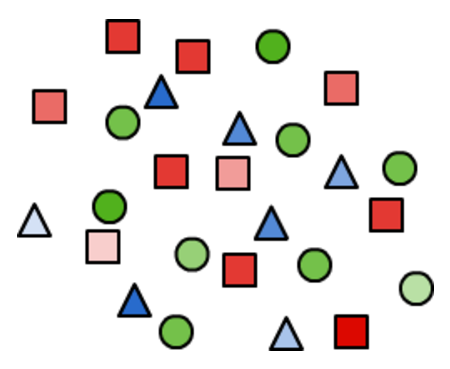
\includegraphics[scale=0.8]{figuras/ungroup-elements.eps}
    \label{fig:ungroup-elements}
    \caption{Elementos não agrupados}
  \end{subfigure}%
  \begin{subfigure}{.5\textwidth}
    \centering
    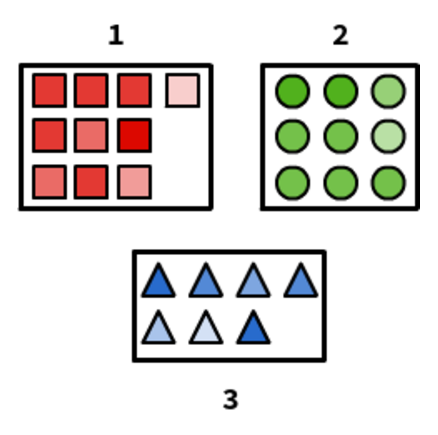
\includegraphics[scale=0.8]{figuras/group-elements.eps}
    \label{fig:group-elements}
    \caption{Elementos agrupados}
  \end{subfigure}
  \caption{Exemplo de clusterização}
\end{figure}

A clusterização é uma técnica da mineração de dados que consiste, justamente, em realizar o procedimento descrito acima: organizar um conjunto de elementos, usualmente representados por vetores ou pontos em um espaço multidimensional, em \textit{clusters} (ou agrupamentos), de acordo com alguma medida de similaridade. Ela representa uma das principais etapas da análise de dados, denominada análise de \textit{clusters} \cite{jain1999}.

Não existe uma técnica de clusterização universal capaz de revelar toda a variedade de estruturas que podem estar presentes em conjuntos de dados multidimensionais. Diferentes algoritmos dependem implicitamente de certas hipóteses a respeito da forma dos clusters, da definição da medida de similaridade e dos critérios de agrupamento \cite{estivill2002}.

\subsubsection{Algorítmo \textit{k-means}}
\label{sub:k_means}

O algorítmo de clusterização \textit{k-means}, proposto por \citeonline{lloyd1957}, tem o objetivo de dividir \(N\) elementos em \(k\) grupos, onde cada elemento pertence ao \textit{cluster} mais próximo. O valor de \(k\) deve ser informado a priori, sendo menor que a quantidade de elementos.

Os passos do algoritmo são:

\begin{enumerate}
  \item \textbf{Gerar centróides:} neste passo os \(k\) centróides recebem valores iniciais. O valor inicial dos centróides podem ser definidos randomicamente, através de uma Gaussiana (com média e variância estimados a partir do conjunto de elementos) ou escolhendo aleatoriamente \(k\) dos \(N\) elementos como centróides iniciais ou definindo-os como centróides de \(k\) grupos escolhidos aleatoriamente a partir dos dados iniciais.
  \begin{figure}[h]
    \centering
    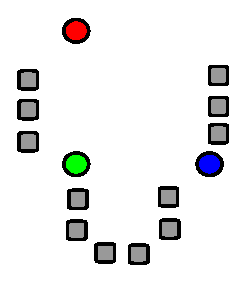
\includegraphics[scale=0.6]{figuras/kmeans-1.eps}
    \caption{k centróides (coloridos) recebem valores iniciais.}
  \end{figure}
  \item \textbf{Calcular distâncias:} aqui são calculadas as distâncias entre cada ponto e cada centróide. É a parte com maior peso computacional do algorítmo, já que o calculo é realizado para cada ponto.
  \item \textbf{Classificar os pontos:} cada ponto deve ser classificado de acordo com a distância entre ele e o centróide de cada \textit{cluster}. O ponto pertencerá ao \textit{cluster} cujo centróide está mais próximo. O algorítmo converge quando, em uma iteração, nenhum ponto mudar de \textit{cluster}.
  \begin{figure}[h]
    \centering
    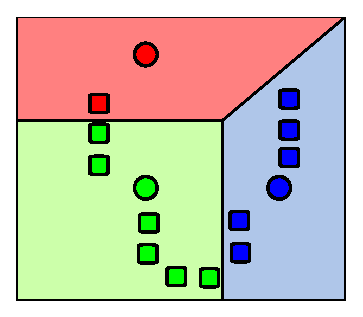
\includegraphics[scale=0.6]{figuras/kmeans-2.eps}
    \caption{Cálculo das distâncias entre os pontos e os centróides.}
  \end{figure}
  \item \textbf{Calcular novos centróides:} para cada \textit{cluster}, um novo centróide é definido como a média de todos os pontos.
  \begin{figure}[h]
    \centering
    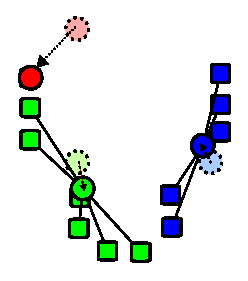
\includegraphics[scale=0.6]{figuras/kmeans-3.eps}
    \caption{Novos centróides definidos pela media dos elementos do \textit{cluster}.}
  \end{figure}
  \item \textbf{Repetir até convergir:} retorna ao passo 2. Como o resultado do algoritmo depende da escolha dos centróides iniciais, a convergência não é garantida ou ele converge para uma solução sub-ótima. Por isso, normalmente o algoritmo é executado várias vezes.
  \begin{figure}[h]
    \centering
    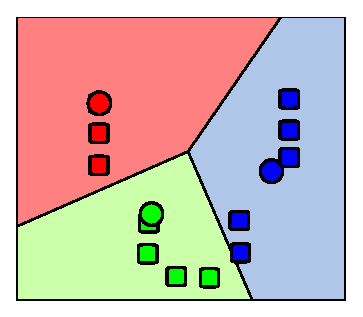
\includegraphics[scale=0.6]{figuras/kmeans-4.eps}
    \caption{O algorítmo converge quando nenhum ponto muda de \textit{cluster}.}
  \end{figure}
\end{enumerate}

Mudanças de escala ou de unidade de medidas para determinadas coordenadas dos elementos podem afetar a análise \cite{cole1998}. Sugere-se, então, que seja feito o processo de normalização (\textit{whitening}) dos dados antes da clusterização. A normalização consiste em ajustar a escala das distâncias de forma que os valores fiquem em intervalos padronizados, normalmente com média nula e variância 1.


\subsubsection{\textit{Latent Dirichlet Allocation - LDA}}

O \textit{LDA} foi proposto por \citeonline{pritchard} em uma aplicação inicial na biologia. Em seu modelo, \citeonline{pritchard} utilizam dados de genótipos multilocus para inferir estruturas populacionais e associar cada indivíduos a uma mistura de populações parentais. Dessa forma, também conseguem estudar zonas híbridas entre as populações e identificar indivíduos migrantes e misturados. A aplicação desse modelo no processamento de linguagem natural foi proposta independentemente por \citeonline{blei}, onde os documentos são tratados como os indivíduos e as populações passam a ser tópicos.

No contexto do processamento de linguagem natural, um documento, ou palavra, pode ser representado por uma mistura de vários tópicos, o que permite uma melhor desambiguação dos termos e uma definição de tópicos mais precisa \cite{girolami}. Usamos como exemplo as seguintes frases:

\begin{enumerate}
  \item Eu \textbf{como peixe}.
  \item \textit{Peixes} são \textit{animais}.
  \item Meu \textit{gato} \textbf{come peixe}.
\end{enumerate}

O \textit{LDA} poderia classificar os termos em \textbf{negrito} como pertencentes ao \textbf{Tópico C}, que poderia ser rotulado como ``\textbf{comida}''. Da mesma forma, as palavras em \textit{itálico} também poderiam ser agrupadas em um \textit{Tópico A}, rotulado como ``\textit{animais}''.

Esse modelo tenta inferir duas tabelas de probabilidade: estrutura (\(P\)) e mistura (\(Q\)). Em \(P\) temos as probabilidades de um termo estar presente em uma frase de cada tópico, sendo que essas probabilidades são independentes entre si. Já em \(Q\), temos as probabilidades de cada documento pertencer à cada tópico, mas, nesse caso, as probabilidades devem somar um total de 100\%. Foram utilizados dados hipotéticos nas tabelas abaixo apenas para ajudar na explicação.

\begin{table}[h]
\centering
\begin{tabular}{|c|c|c|}
\hline
\textbf{Termo/Tópico} & \textbf{Comida} & \textbf{Animal} \\ \hline
comer & 0.9 & 0.3 \\ \hline
peixe & 0.5 & 0.6 \\ \hline
animal & 0.2 & 0.8 \\ \hline
gato & 0.2 & 0.8 \\ \hline
\end{tabular}
\caption{Tabela de Estrutura dos Termos (P)}
\label{tabelap}
\end{table}

\begin{table}[h]
\centering
\begin{tabular}{|c|c|c|}
\hline
\textbf{Documento/Tópico} & \textbf{Comida} & \textbf{Animal} \\ \hline
Frase 1 & 0.8 & 0.2 \\ \hline
Frase 2 & 0.1 & 0.9 \\ \hline
Frase 3 & 0.6 & 0.4 \\ \hline
\end{tabular}
\caption{Tabela de Mistura dos Documentos (Q)}
\label{tabelaq}
\end{table}

Essas tabelas influenciam diretamente uma à outra, ou seja, se um termo começa a ser predominante em determinado tópico, o documento a qual ele pertence passa a tender à esse tópico. Da mesma forma que se um documento começar a tender a um tópico, seus termos também serão favorecidos neste tópico.

Para se obter o conteúdo de cada tópico, basta observar as colunas de \(P\), onde teremos uma \textit{bag of words} contendo a probabilidade de todos os termos pertencerem à esse tópico. Analisando as linhas de \(Q\), temos as misturas de tópicos de cada documento. Vale notar que, por ser uma mistura de tópicos, o \textit{LDA} dificilmente vai atribuir um documento à um único tópico com 100\% de pertencimento.

Para chegar à essa conclusão, o \textit{LDA} segue três passos:

\paragraph{Quantidade de Tópicos}
Assim como no \textit{k-means}, o primeiro passo é definir a quantidade de tópicos que serão obtidos ao final da análise. Esse número pode ser obtido através de uma análise prévia dos dados ou simplesmente por uma escolha aleatória.

\paragraph{Inicializar as tabelas \(P\) e\(Q\)}
É definida uma distribuição de tópico inicial para cada documento, que será atualizado no passo seguinte. A escolha desses tópicos se dá de forma semi-aleatória, de acordo com a distribuição de \textit{Dirichlet}, ou seja, valores aleatórios entre 0 e 1 com a restrição de que a soma deles deve ser 1. As probabilidades \(P\) podem ser definidas de forma uniforme para todos os termos: \(P=0.5\).

\paragraph{Analisar e Atualizar os Tópicos}
Para cada palavra, em todos os documentos, a definição do tópico é atualizada de acordo com dois critérios: quão essa palavra é predominante  entre os tópicos e quão predominante são os tópicos entre as palavras do documento. Em outras palavras, as probabilidades são recalculadas fixando os valores de \(P\) para obter os novos valores de \(Q\) e, em seguida, fixa-se os valores de \(Q\) para recalcular as probabilidades de \(P\). Dependendo do algoritmo esse processo pode ser repetido para cada palavra e em todos os documentos, passando por todo o \textit{corpus} várias vezes até convergir \cite{annalyn}.

\clearpage
\section{Aprendizado Semi-Supervisionado}

Essa forma de aprendizado é útil quando quando existem apenas alguns exemplos já classificados e pode ser utilizado tanto em tarefas de classificação quanto em tarefas de \textit{clustering}. A ideia do aprendizado semi-supervisionado é utilizar esses exemplos previamente classificados para se obter informações sobre o problema e utilizá-las para auxiliar o processo de aprendizado a partir de exemplos não classificados \cite{bruce}.

Existem várias estratégias para definir algoritmos de aprendizado semi-supervisionado. É comum utilizar modelos de aprendizado não-supervisionado com alterações, afim de se poder inserir informações a priori.

Podemos tornar o algoritmo \textit{k-means} semi-supervisionado se fixarmos \textit{clusters} específicos para determinados termos previamente classificados, de forma que esse eles sempre pertençam aos \textit{clusters} pré-fixados. Dessa forma, a informação inserida influenciará diretamente na posição dos \textit{clusters}.

No \textit{LDA}, também podemos fixar algumas linhas da tabela de mistura \(Q\). Dessa forma, podemos dizer que um texto pertence a um tópico específico ou a misturas específicas de tópicos.


\section{Distância entre os pontos}
\label{ssub:distância_entre_os_pontos}

Segundo \citeonline{cole1998}, para clusterizar termos de acordo com sua similaridade, deve-se definir uma medida de quão próximos dois termos estão. Uma medida de distância (métrica) deve ser definida de tal forma que:

\begin{itemize}
  \item Seja sempre positiva.
  \item Seja simétrica: a distância de um termo \(A_{i}\) para um termo \(A_{j}\) deve ser a mesma de \(A_{j}\) para \(A_{i}\).
  \item Seja reflexiva: se a distância entre \(A_{i}\) e \(A_{j}\) é zero, então \(A_{i} = A_{j}\).
  \item Respeite a desigualdade triangular: considerando os termos (\(A_{i}, A_{j}\) e \(A_k\)), a distância \(d(A_{i}, A_k)\) deve ser menor ou igual à soma das distâncias \(d(A_{i}, A_{j})\) e \(d(A_{j}, A_k)\)
\end{itemize}

Existem várias medidas de distância. Começamos pela distância Euclidiana entre dois pontos, \(A=(a_1, a_2, a_3, \ldots, a_n) \) e \(B=(b_1, b_2, b_3, \ldots, b_n) \), dada pela equação
%
\begin{align}
  dist(A, B) &= \sqrt{\displaystyle\sum_{i=1}^{n} (a_i-b_i)^2} \label{eq:euclidean}
\end{align}

Já a distância de Manhattan entre dois pontos, \(A=(a_1, a_2, a_3, \ldots, a_n) \) e \(B=(b_1, b_2, b_3, \ldots, b_n) \), é dada pela soma das diferenças absolutas de suas coordenadas:

\begin{align}
  dist(A, B) &= \displaystyle\sum_{i=1}^{n} |a_i-b_i| \label{eq:manhattan}
\end{align}

Em ambos os casos, temos que a distância entre do ponto A ao ponto B é a mesma distância do ponto B ao ponto A.

\begin{figure}[h]
  \centering
  \begin{subfigure}{.5\textwidth}
    \centering
    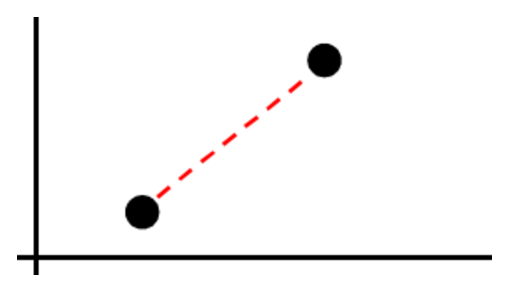
\includegraphics[scale=0.5]{figuras/euclidean.eps}
    \caption{Distância Euclidiana}
  \end{subfigure}%
  \begin{subfigure}{.5\textwidth}
    \centering
    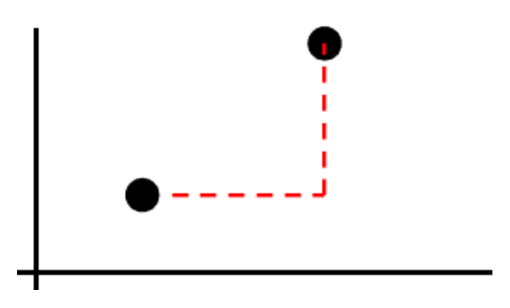
\includegraphics[scale=0.5]{figuras/manhattan.eps}
    \caption{Distância de Manhattan}
  \end{subfigure}
  \caption{Comparação entre distância Euclidiana e de Manhattan}
\end{figure}

Cada métrica pode gerar resultados diferentes no algoritmo \textit{k-means} e normalmente podem ser interpretadas do ponto de vista estatístico como uma escolha do modelo que gerou cada \textit{cluster}. A distância euclidiana pode ser associada a um modelo Gaussiano para gerar os pontos observados onde a média corresponde ao centróide de cada \textit{cluster} e o desvio padrão é o mesmo para todos os grupos.

\subsection{Validação Cruzada}

A validação cruzada é uma técnica geralmente utilizada para avaliar modelos preditivos, buscando estimar o quão preciso é o modelo avaliado. A ideia principal da validação cruzada consiste em dividir o conjunto de dados em subconjuntos mutualmente exclusivos, onde alguns desses subconjuntos serão utilizados para a estimação dos parâmetros do modelo (treinamento) e os outros subconjuntos serão utilizados para a validação do modelo (validação ou teste) \cite{kohavi1995}.

O método \textit{holdout} é uma forma de validação de cruzada comumente utilizada e consiste em dividir o conjunto de dados em dois subconjuntos mutualmente exclusivos, onde seus tamanhos podem, ou não, ser diferentes. Um subconjunto servirá para o treinamento do modelo e o outro para a sua validação. Uma proporção comum é considerar 2/3 dos dados para treinamento e 1/3 para a validação. Essa abordagem é indicada quando está disponível uma grande quantidade de dados. Quando o conjunto de dados é muito pequeno, o erro calculado na predição pode sofrer muita variação \cite{kohavi1995}.

Uma das métricas mais simples para avaliar o modelo é a comparação item a item dos resultados esperados pelos resultados obtidos:
%
\begin{align}
P_{a}=\frac{N_{vp}}{N_{it}},
\end{align}
%
onde \(P_{a}\) é a porcentagem de acertos do modelo, \(N_{vp}\) é o número de itens classificados corretamente pelo modelo e \(N_{it}\) é o número total de itens que fazem parte do conjunto de testes.

